\chapter{Identifying Types of Load from Standing Wave Pattern\index{standing wave pattern}}\label{lec:lec9}

In the previous chapter, we discussed how to solve some simple common transmission line problems using both impedances and admittances and then we discussed the constant VSWR circle. In this chapter, we will discuss how to identify the types of load from standing wave patterns. Standing wave pattern has two important characteristics which are:
\begin{enumerate}[(i)]
\item The location of maximum and minimum (current/voltage)
\item The VSWR circle.
\end{enumerate}
So \emph{how can we quickly identify the type of load\footnote{The type of load is not the exact value of the load} without calculating the VSWR?}

Recall that:
\begin{align}
VSWR = \frac{|V|_\max}{|V|_\min}
\label{eqn:vswr09}
\end{align}
From the equation~\eqref{eqn:vswr09}, the smaller the value of $|V|_\min$, the larger the value of ${VSWR}$, that is, as $|V|_\min$ tends to zero, ${VSWR}$ tends to infinity. When $|V|_\max{\approx}|V|_\min$, then $VSWR = 1$.

First, let us observe the variation of the impedance on the tranmission line with the Smith Chart then we will revisit our early question. Figures~\ref{fig:group91} and~\ref{fig:group92} are simplified Smith Charts showing the VSWR circle for inductive and capacitive load at the top and bottom areas respectively.
\begin{figure}[h]
\centering
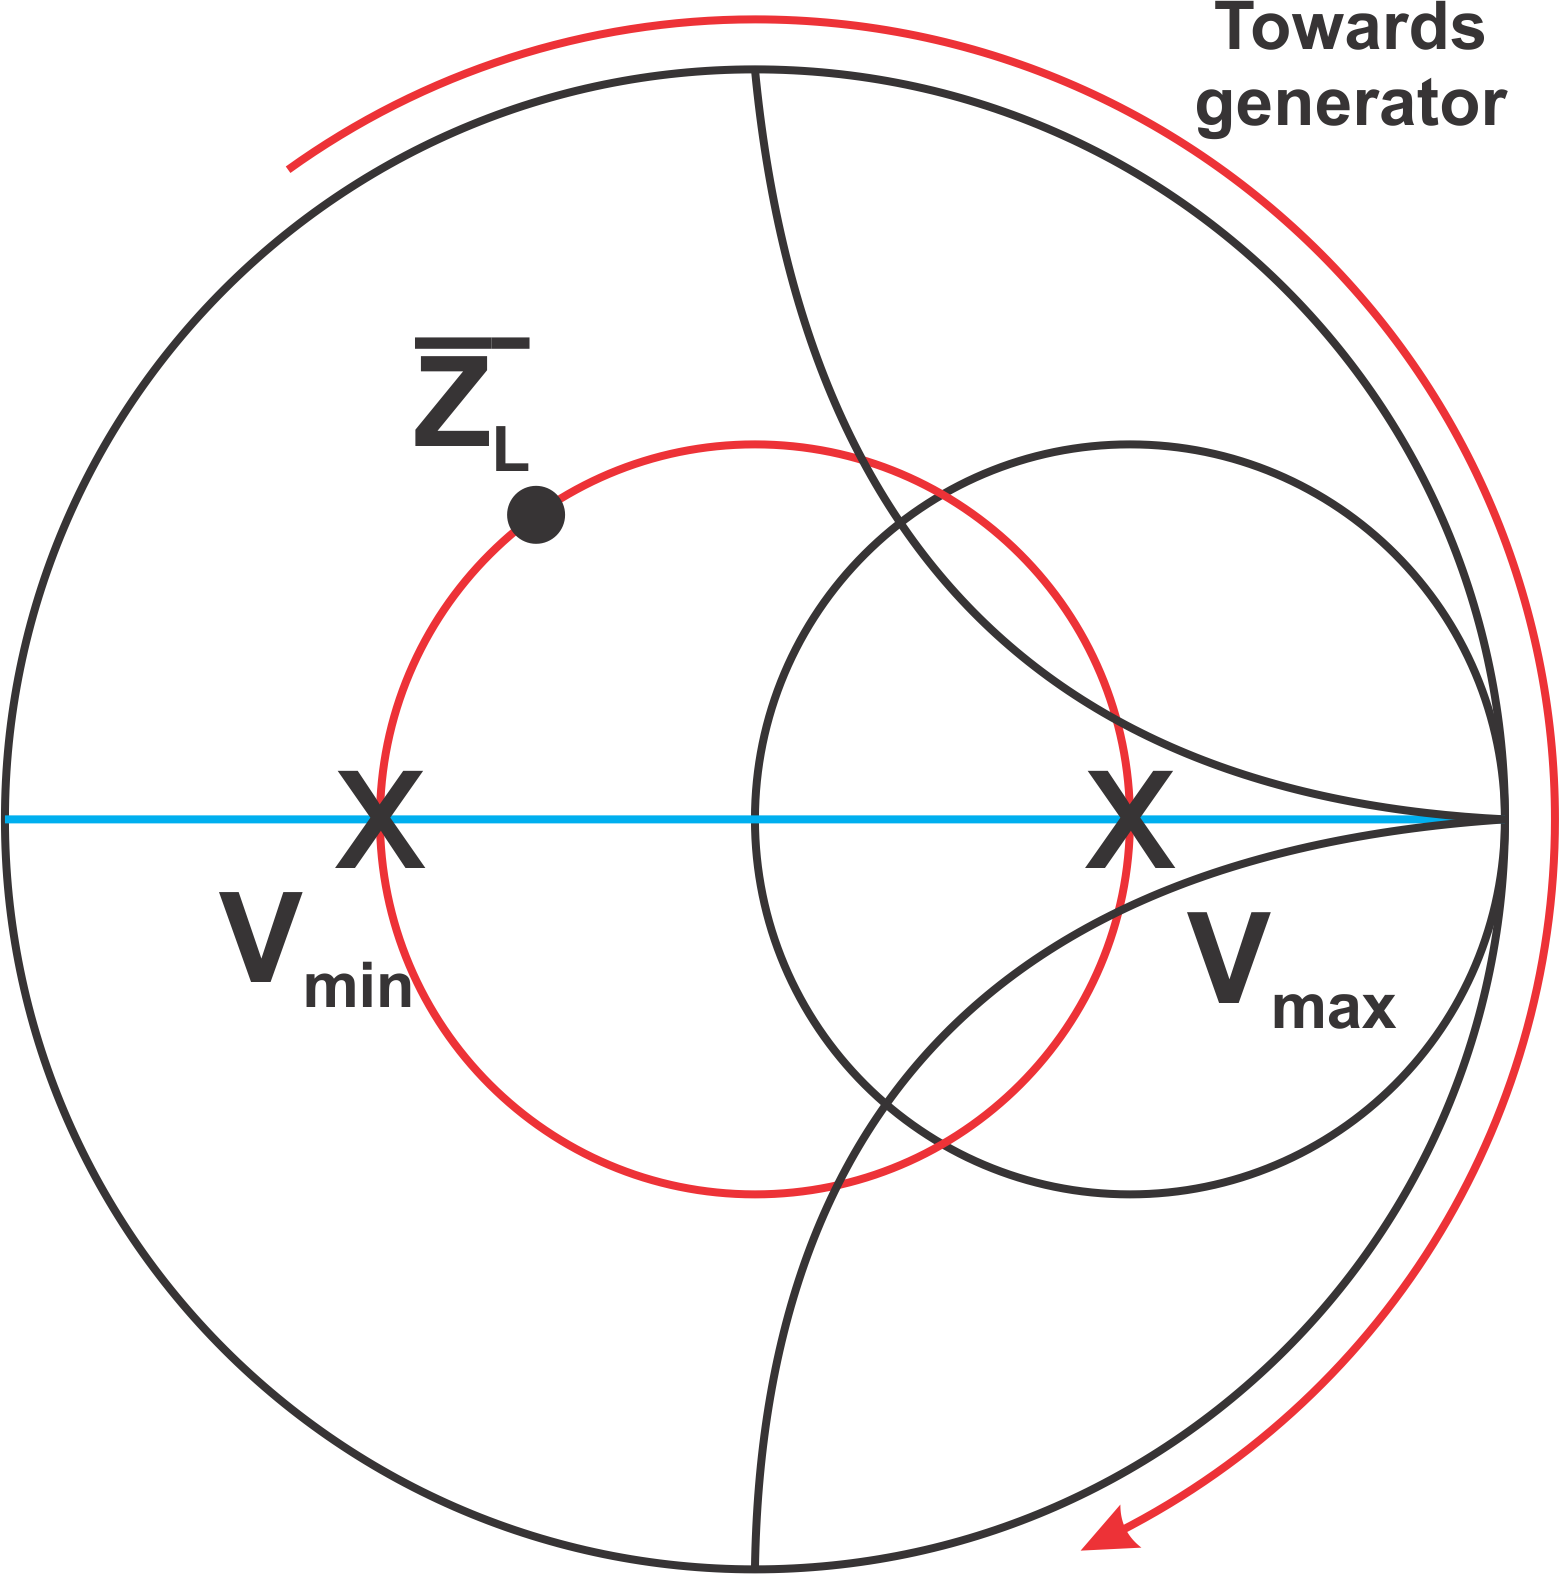
\includegraphics[scale=0.4]{./graphics/Group91}
\caption{A Smith Chart representation of inductive load}
\label{fig:group91}
\end{figure}
\begin{figure}[h]
\centering
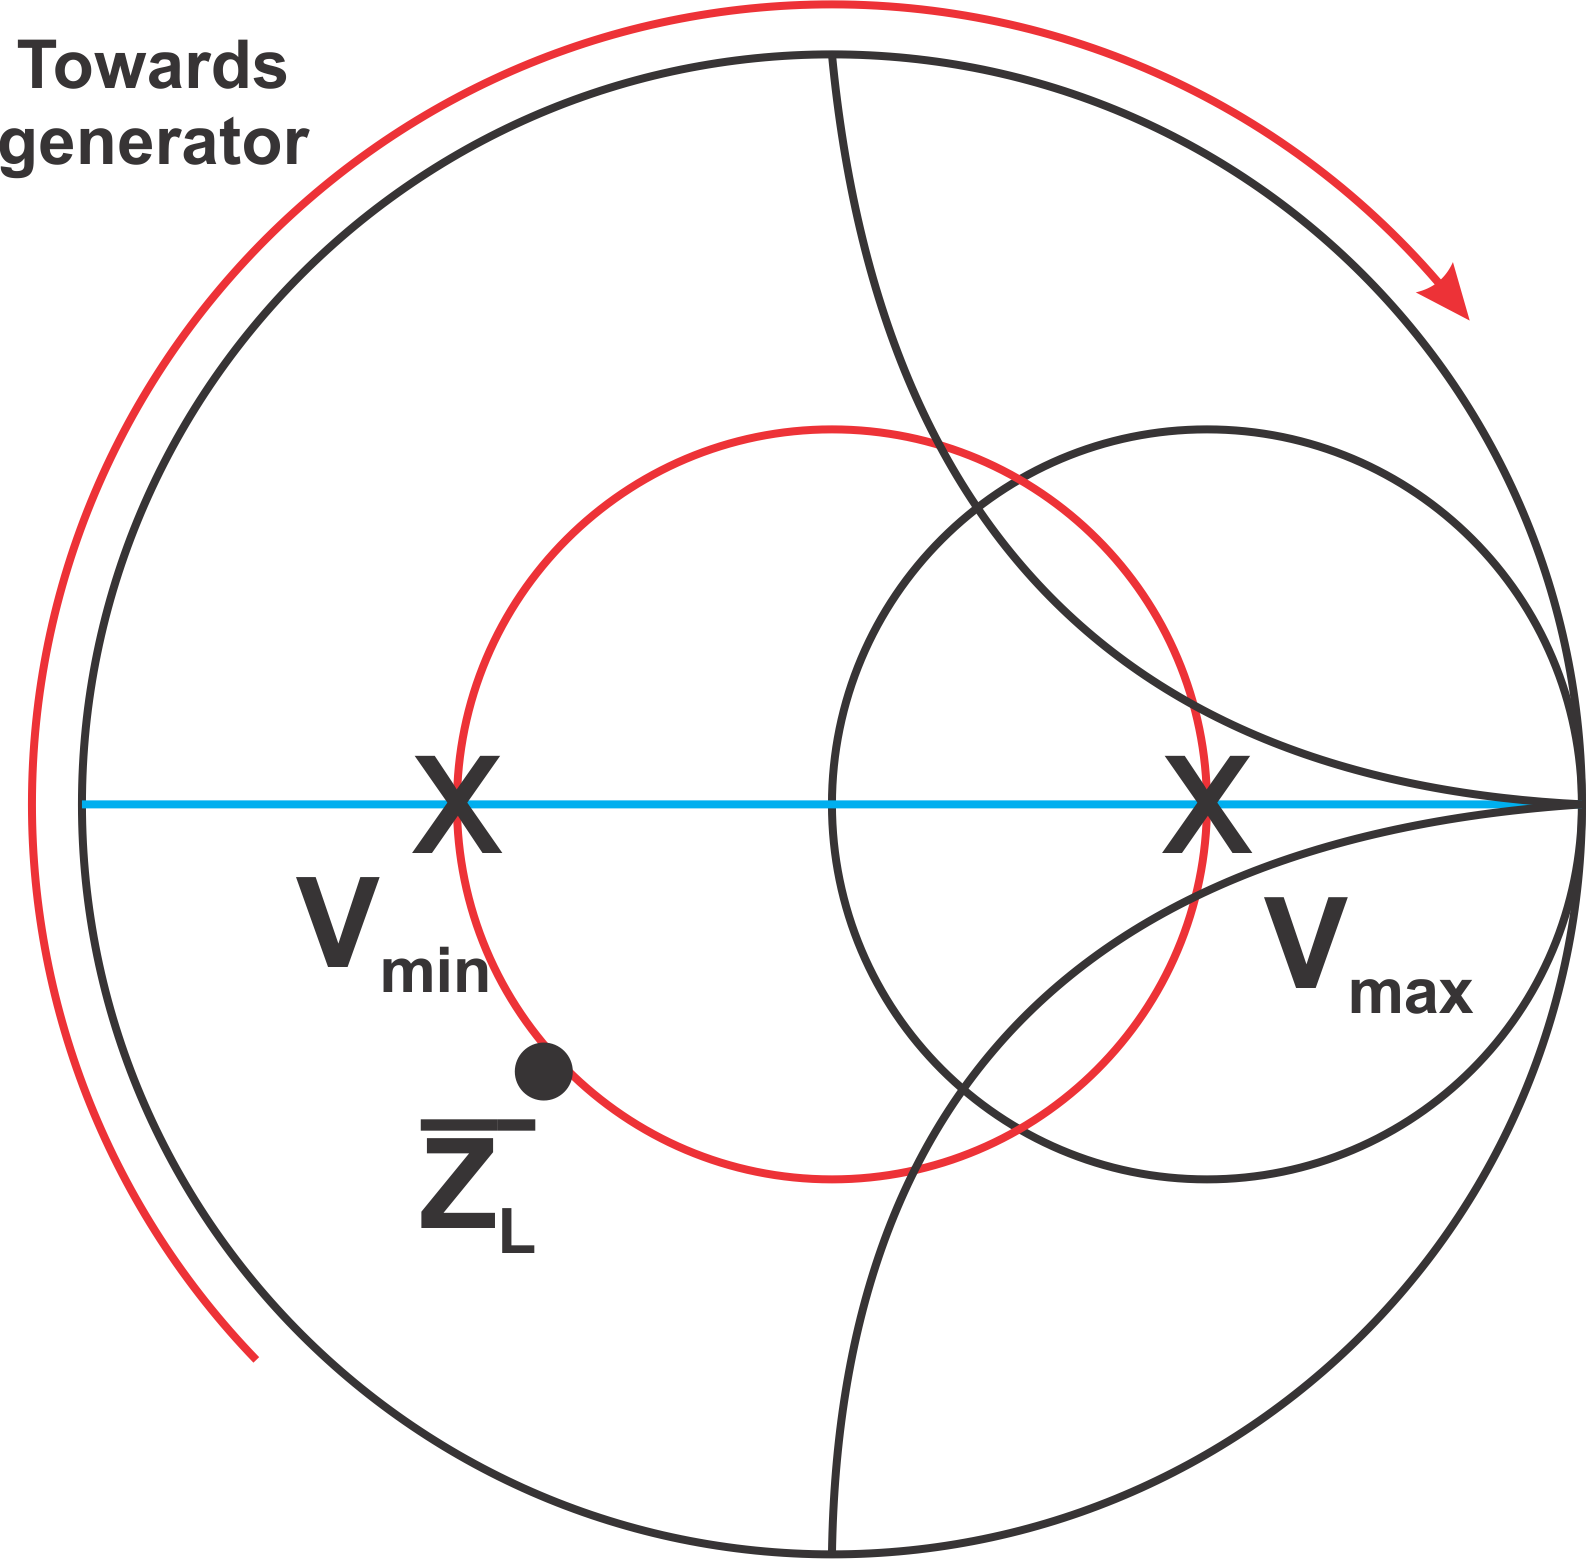
\includegraphics[scale=0.4]{./graphics/Group92}
\caption{A Smith Chart representation of capacitive load}
\label{fig:group92}
\end{figure}

As shown in figure~\ref{fig:group91}, if we move from the load towards the generator, that is, a clockwise rotation, for the inductive load we encounter $V_\max$ first before ${V_\min}$ in another $\frac{\lambda}{4}$ or $\pi rad$ movement. Similarly, if we move from $\bar{Z_L}$ in clockwise direction for capacitive load, we encounter $V_\min$ first before $V_\max$, in another $\frac{\lambda}{4}$ or $\pi rad$ movement. Also, $V_\min\neq0$ which means that for a complex inductive load that is not purely reactive, $VSWR\neq\infty$.

\section{Complex Reactive Loads}
Now, let us analyze some standing wave graph and determine the type of load which they represent. The transmission line circuit is shown in figure~\ref{fig:group93} and we can analyse the standing wave pattern based on the new observation we have discussed. As the standing wave pattern moves from load towards the generator from right to left, it gets to a maximum first and its minimum is not zero so it $|V_\min|$ does not touch the real axis.
\begin{figure}[h]
\centering
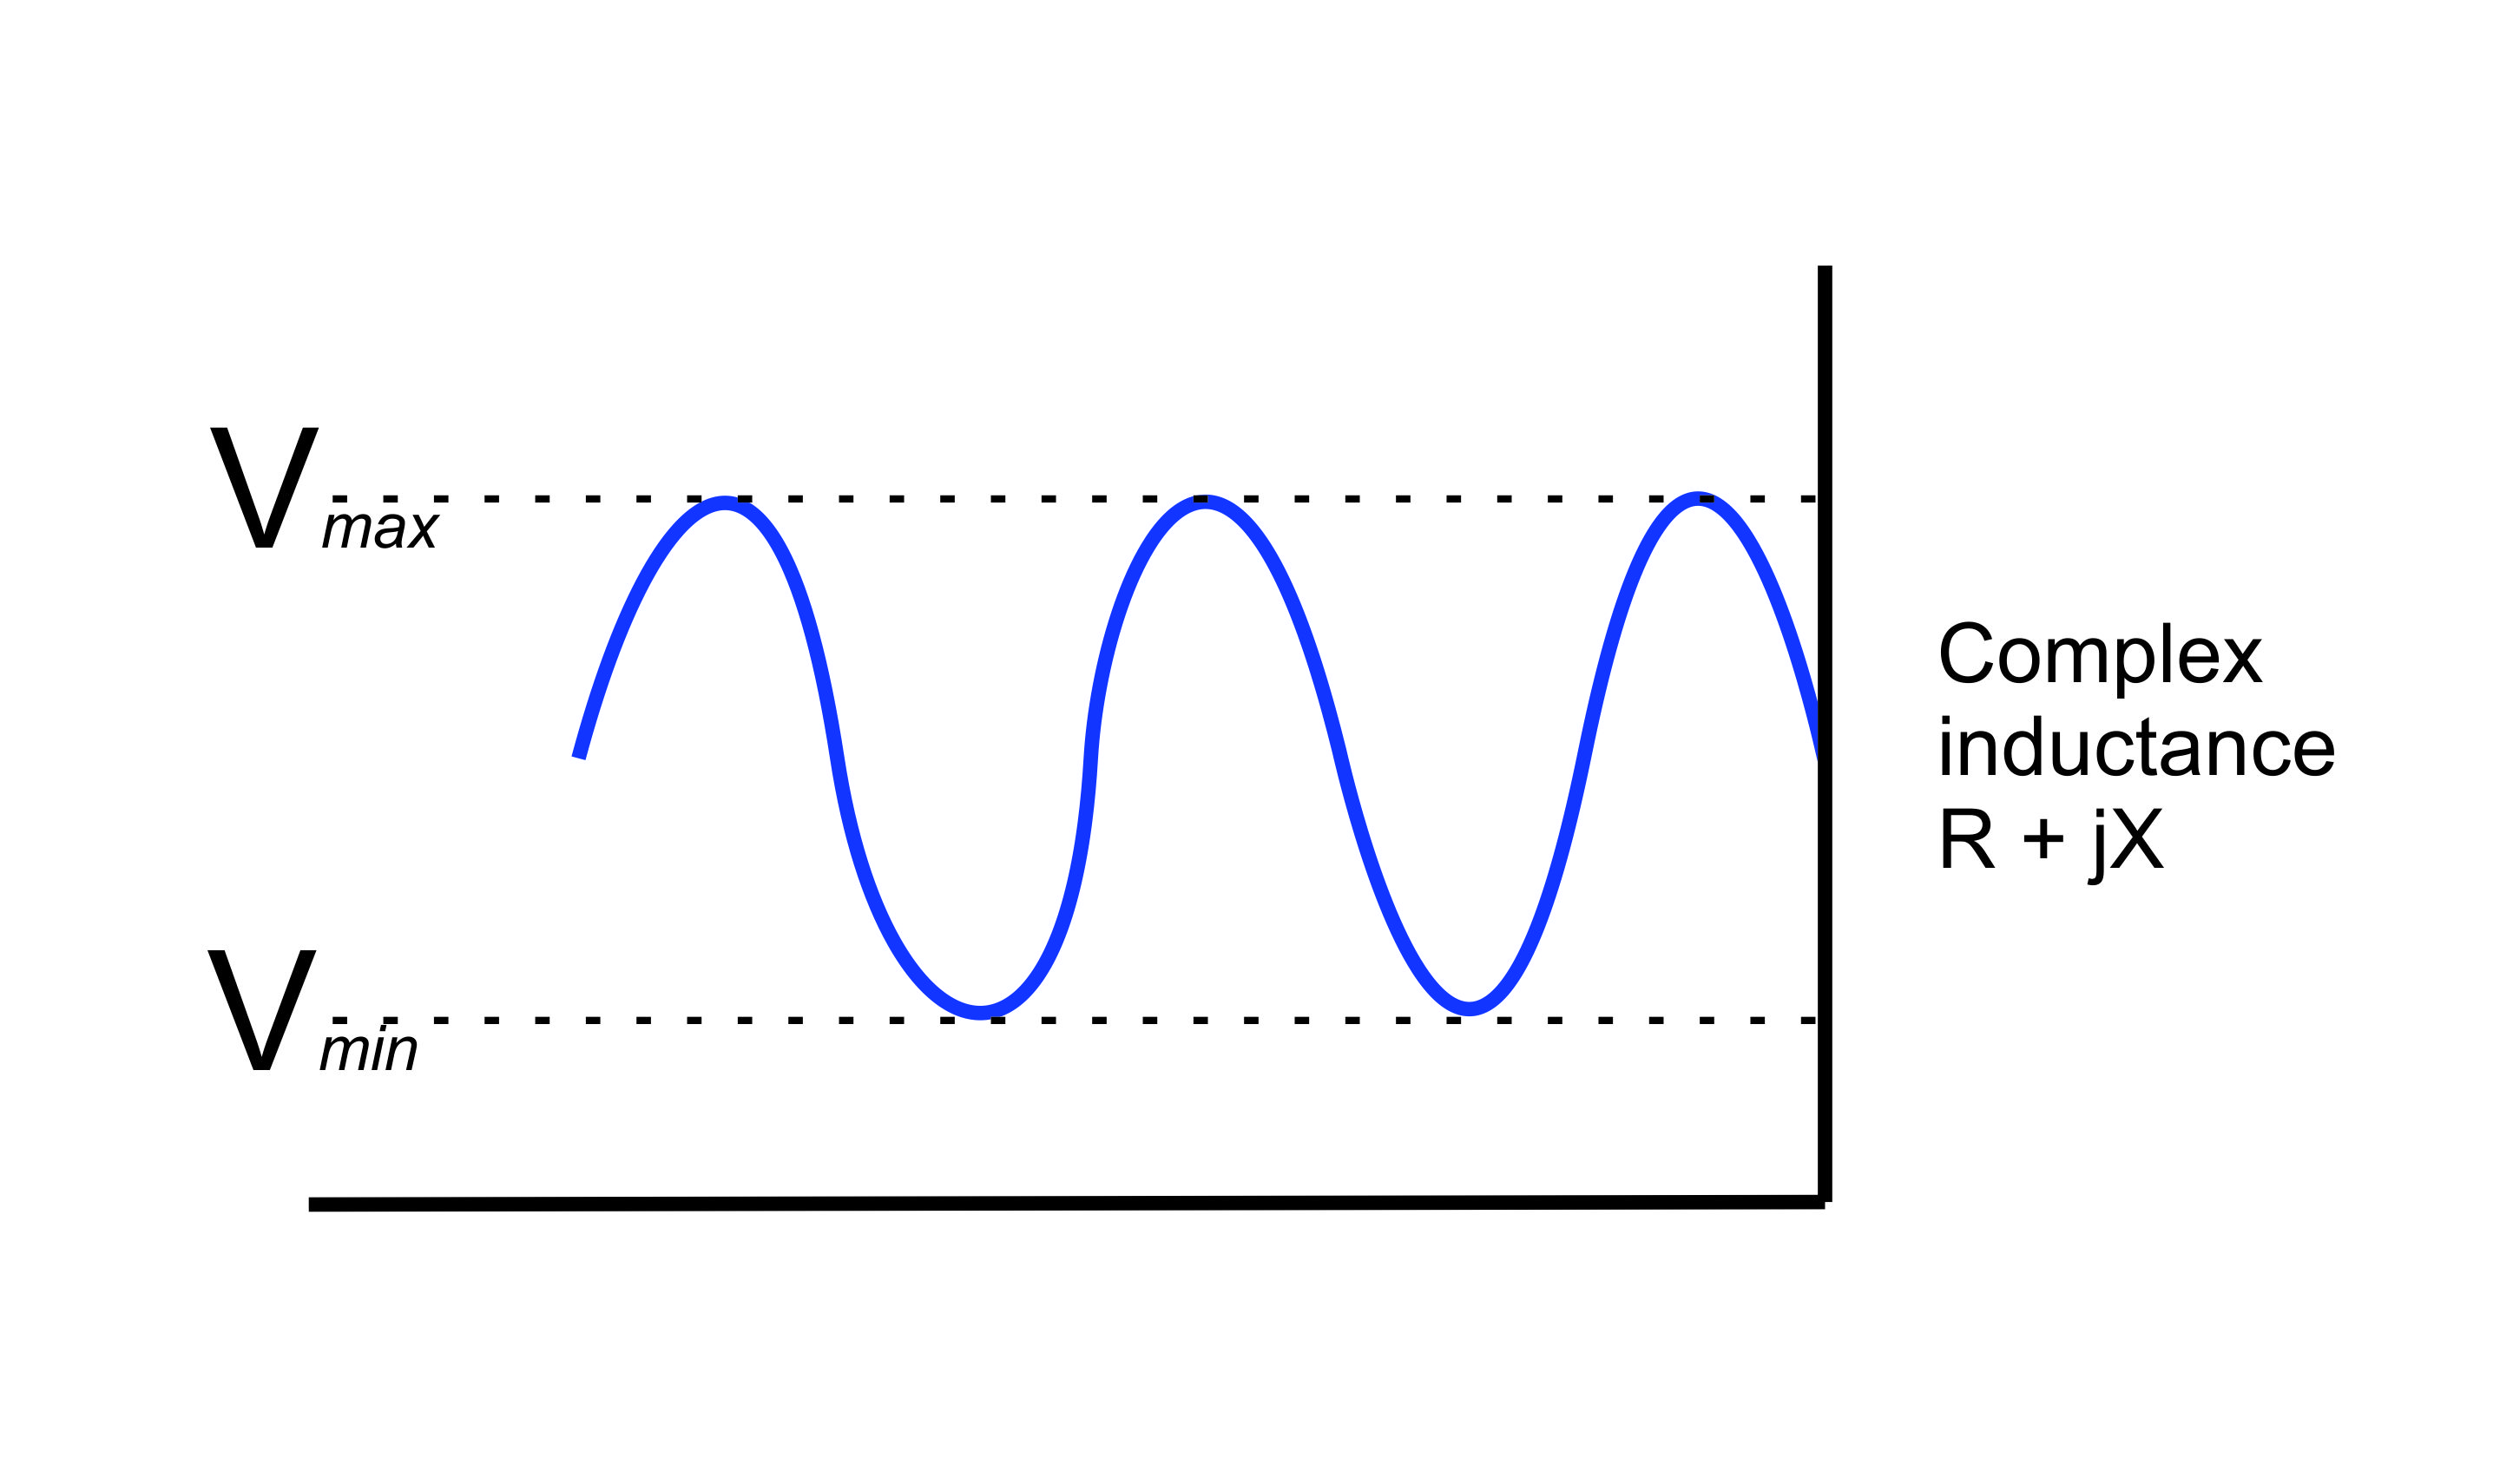
\includegraphics[scale=0.5]{./graphics/Group93}
\caption{Standing wave pattern variation of a complex inductive load}
\label{fig:group93}
\end{figure}
\begin{figure}[h]
\centering
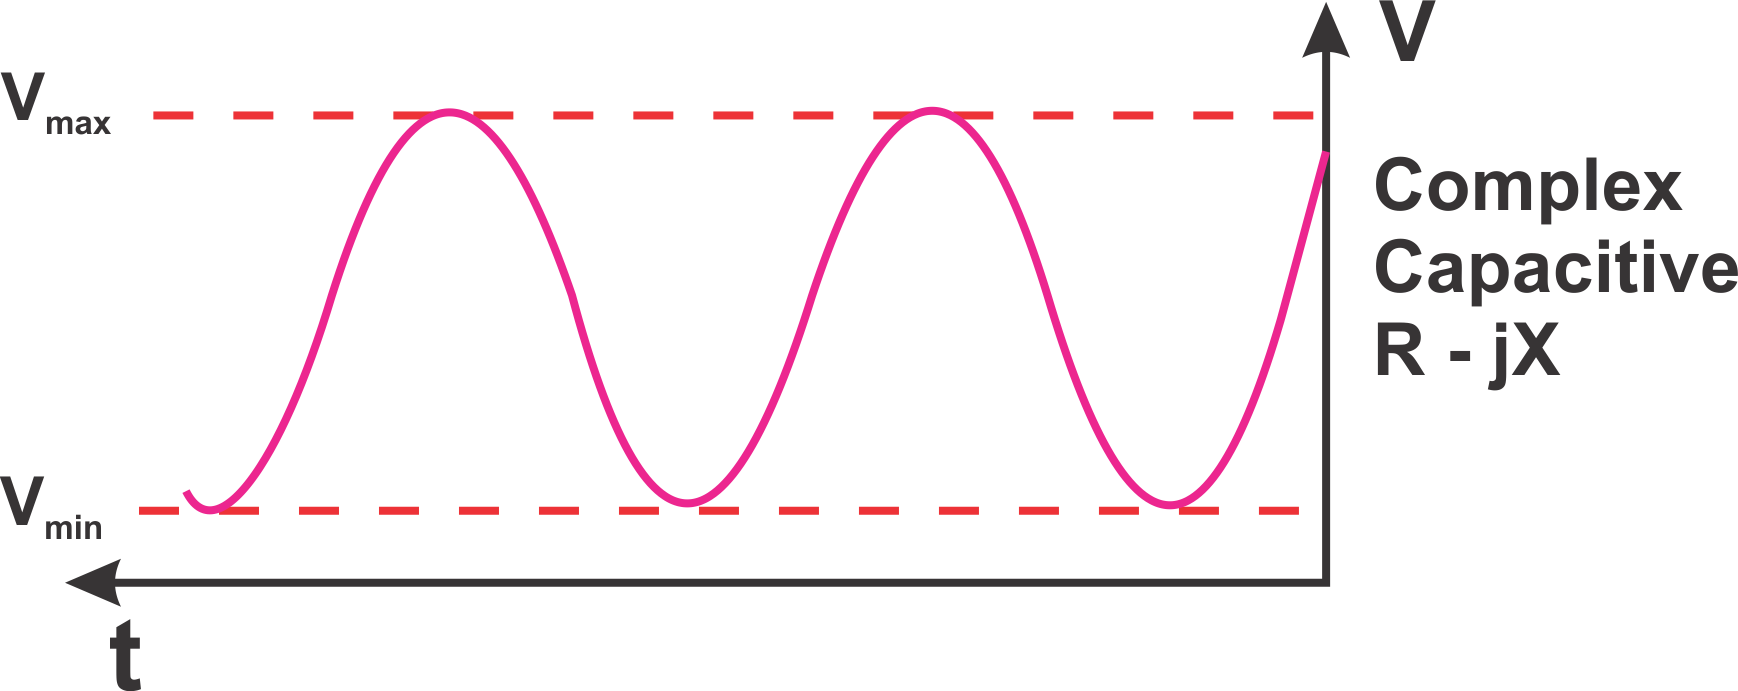
\includegraphics[scale=0.5]{./graphics/Group94}
\caption{Standing wave pattern variation of a complex capacitive load}
\label{fig:group94}
\end{figure}

Similarly for a complex capacitive load, $V_\min\neq0$ and we encounter $V_\min$ first before $V_\max$ as shown in figure~\ref{fig:group94}. 

\section{Purely Reactive Loads}
Let us observe the standing wave patterns with pure reative components at the load end. As shown in figure~\ref{fig:group96}, the voltage minimum is zero or it touches the horizontal axis that is ${VSWR=\dfrac{V_\max}{V_\min}=\infty}$ as ${V_\min=0}$.
\begin{figure}[h]
\centering
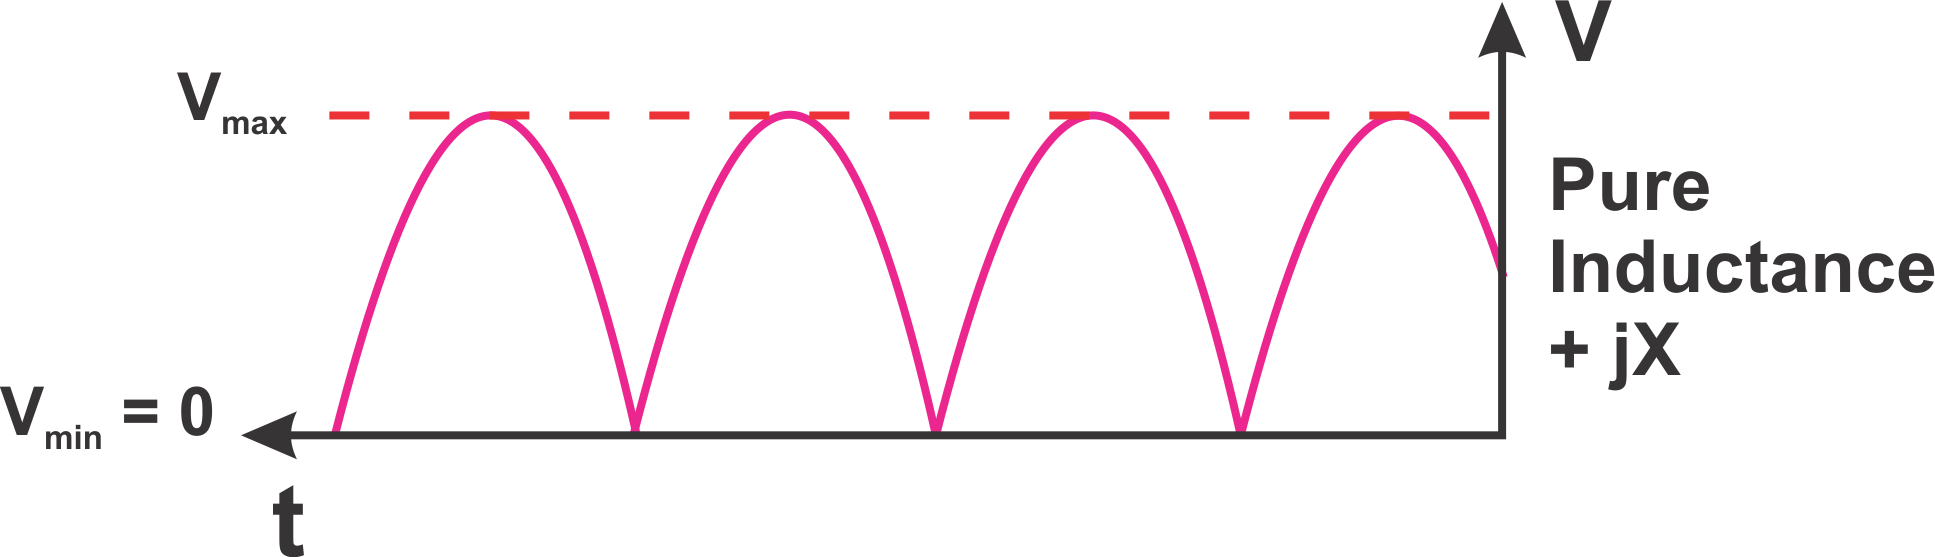
\includegraphics[scale=0.5]{./graphics/Group96}
\caption{Standing wave pattern variation of a pure inductive load}
\label{fig:group96}
\end{figure}

As we move from the load end we meet ${V_\max}$ first indicating it is purely inductive and lies on the upper half of the Smith Chart.
\begin{figure}[h]
\centering
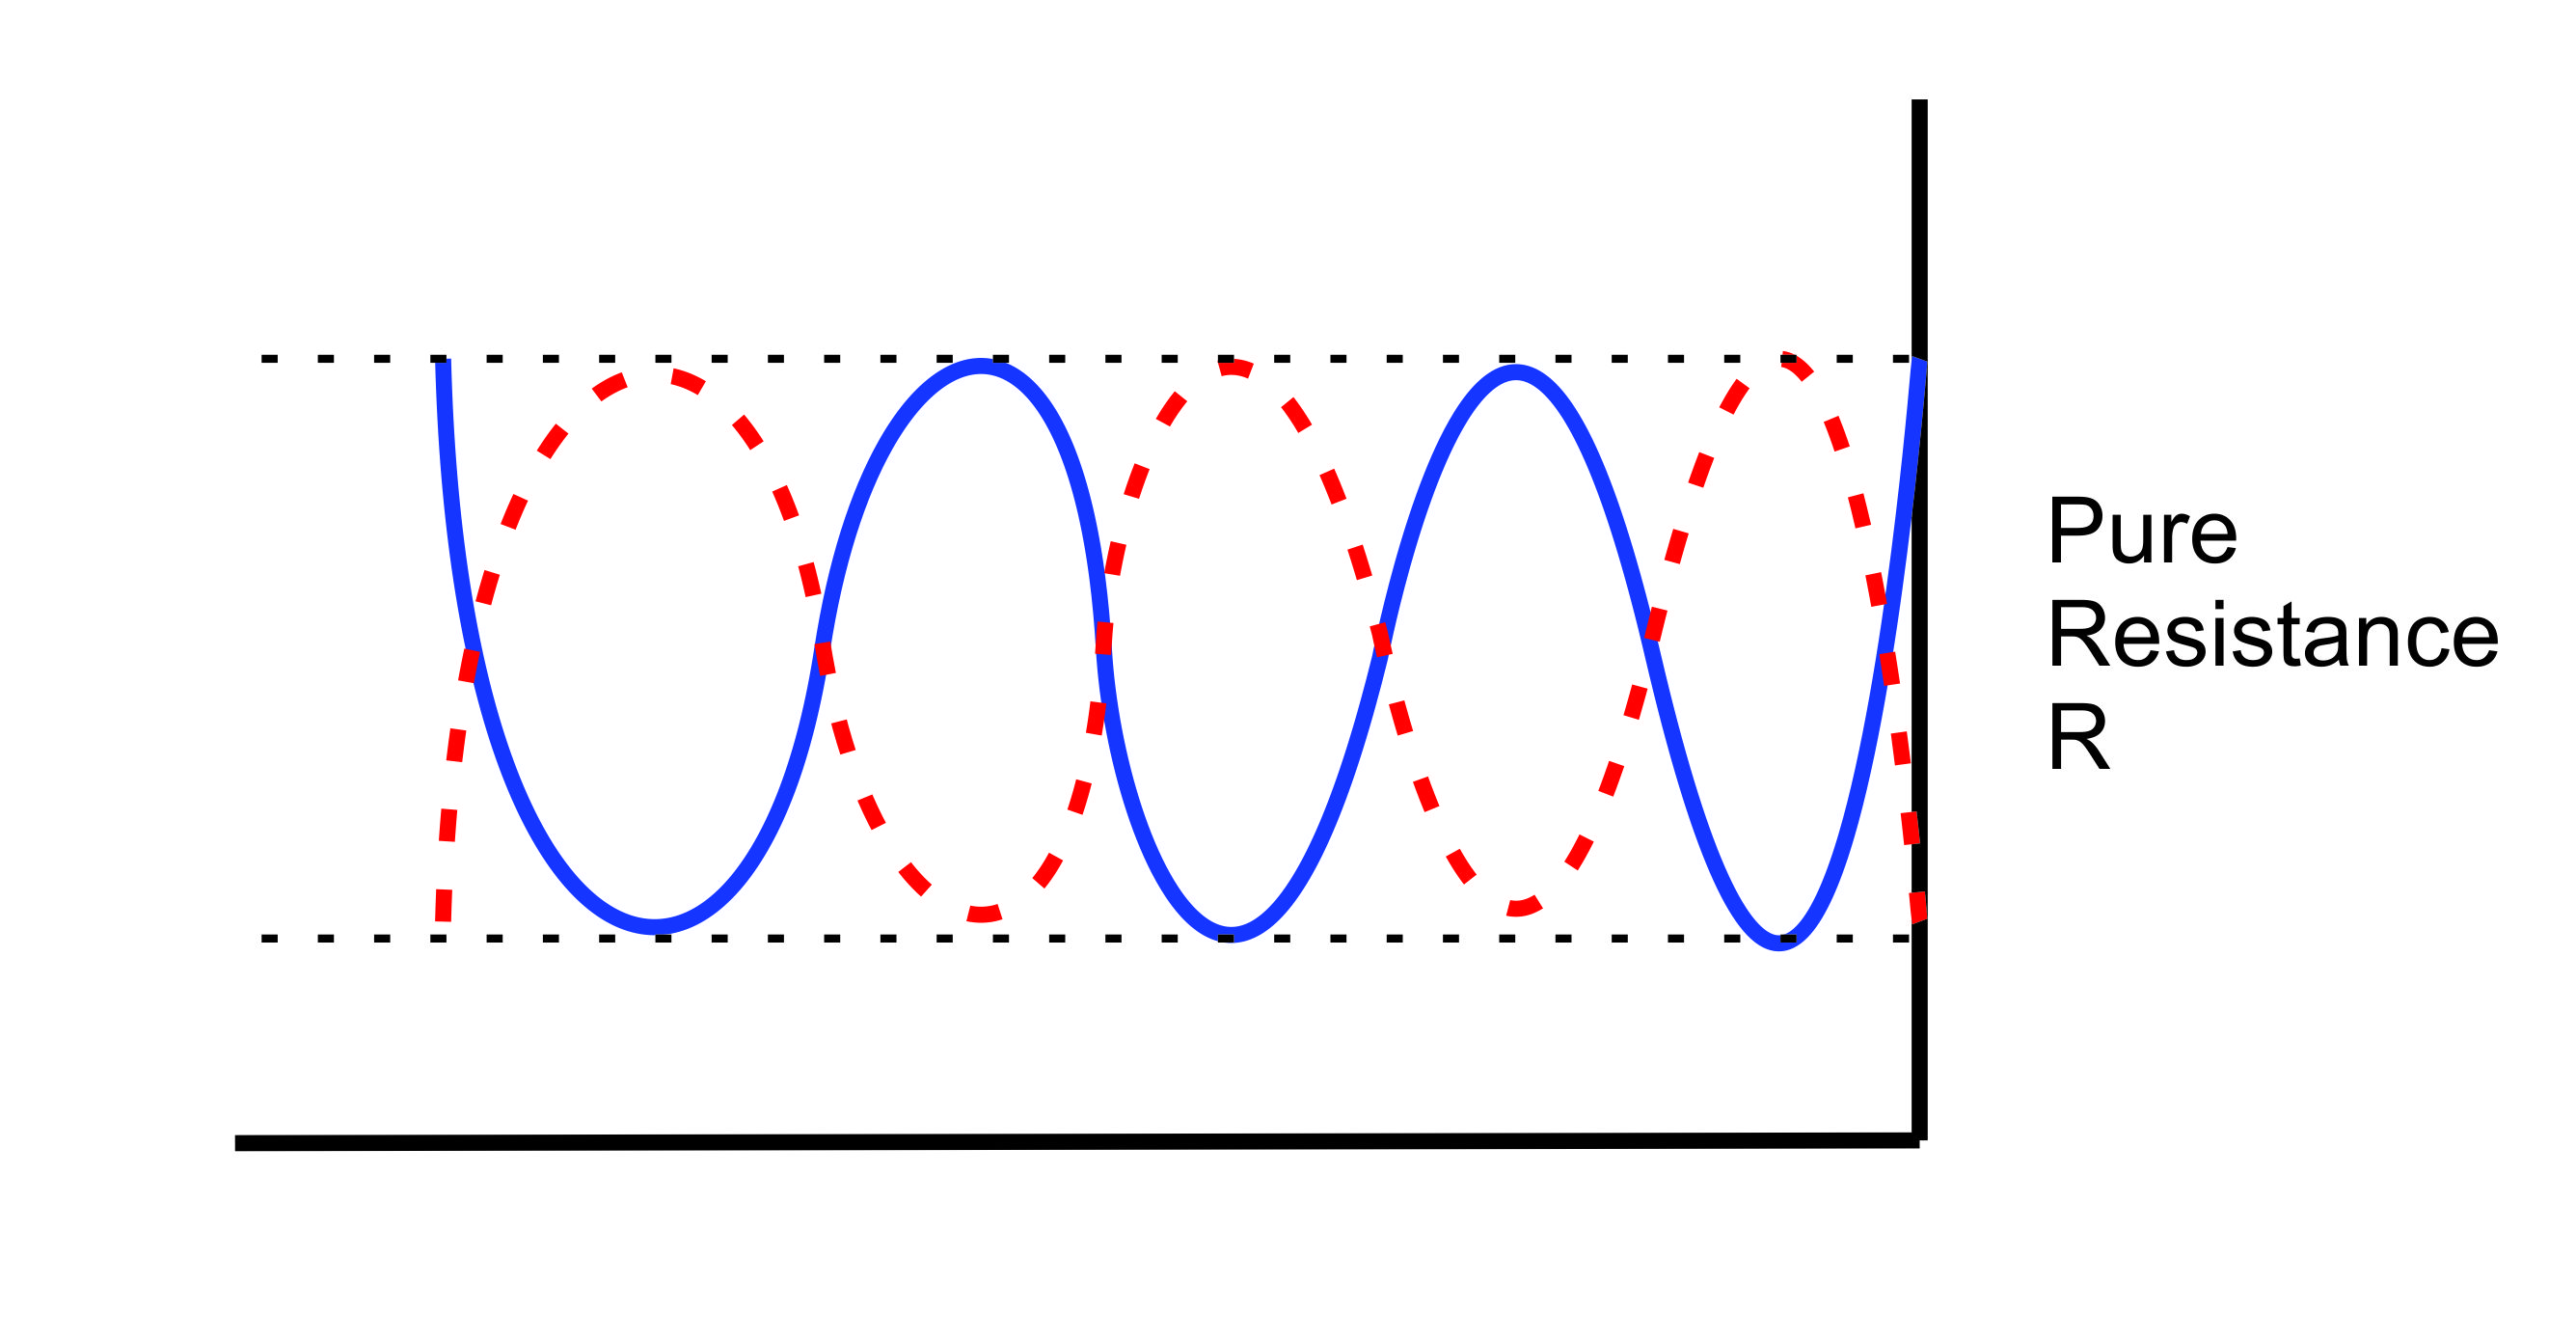
\includegraphics[scale=0.5]{./graphics/Group97}
\caption{Standing wave pattern variation of a pure capacitive load}
\label{fig:group97}
\end{figure}

For purely capacitive loads, the voltage minimum is also zero, but we encounter a minimum first as we go from the load end towards the generator indicating a purely capacitive load. So it lies in the lower half of the Smith Chart and $VSWR=\infty$.

\section{Resistive Loads}
Lastly, there is the case of when the load is neither capacitive nor inductive. If so, then the load must lie on the real horizontal axis of the Smith Chart, so the location of the load itself will be at either the voltage minimum point or voltage maximum point. If the load is purely resistive as in figure~\ref{fig:group95}. Recall that on the Smith Chart, the points of intersection of the VSWR circle on the real axis will be the locations of the voltage maximum and minimum. So there will either be maximum or minimum voltage at the load end as shown in figure~\ref{fig:group95}. The solid curve has ${V_\max}$ at load end meaning ${R>Z_o}$ while the dashed curve has ${V_\min}$ at load end which means ${R<Z_o}$. ${Z_o}$ is the characteristics impedance.
\begin{figure}[h]
\centering
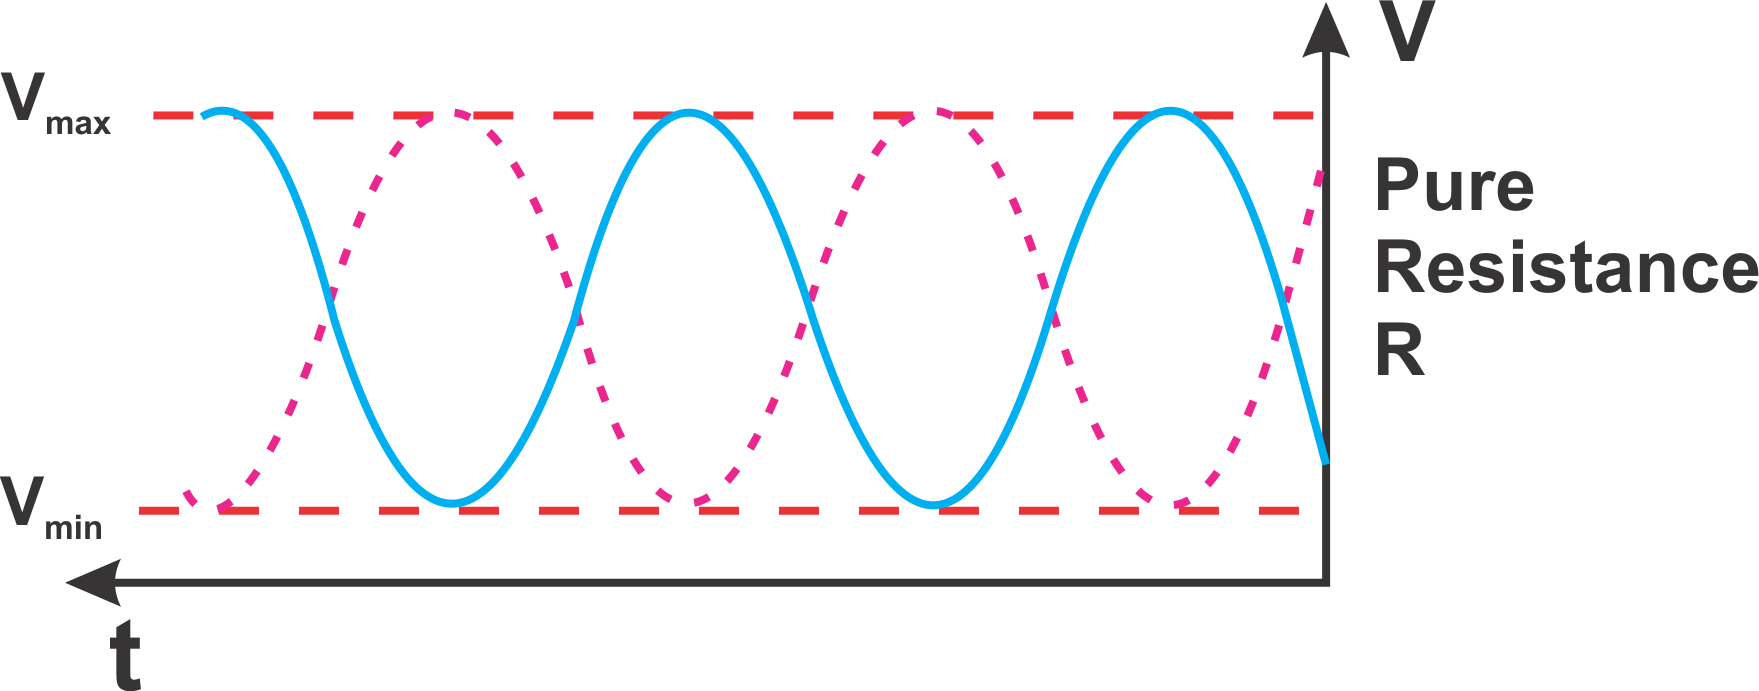
\includegraphics[scale=0.5]{./graphics/Group95}
\caption{Standing wave pattern variation of a pure resistive}
\label{fig:group95}
\end{figure}

So looking at the standing wave pattern, one can quickly identify the types of load because the information about the load is completely available from the standing wave pattern. Hence, ${V_\max}$ and ${V_\min}$ location and lowest value of ${V_\min}$ which is related to VSWR can help us identity loads very quickly.

\section{Transmission line problems}
Now we solve some simple problems based on the theory we have developed from the transmission line.

\begin{exmp}
A voltage wave at ${1GH}z$ is traveling on a transmission line in ${+x}$ direction. The primary constants of the line are ${R=0.5\Omega/m}$, ${L=0.2\mu H/m}$, ${G=0.1\upsilon/m}$, ${C=100pF/m}$. Calculate the attenuation constant in ${nepers/m}$ and ${dB/m}$. If the voltage of the forward traveling wave at ${t=0}$ and ${x=0}$ ${v}=0.866V$. Find the voltage at ${x=1m}$ and time ${t=100nsec}$. What is the peak voltage at ${x=1m?}$ Take initial phase as ${30^0}$.

\subsection*{Solution}
\[\omega = 2\pi\times 10^{9}\text{rad/sec}\]
Propagation constant $\gamma = \sqrt{(R + \jmath\omega L)(G + \jmath\omega C)}$
\begin{dmath*}
\gamma
=\sqrt{(0.5 + \jmath( 2\pi\times 10^{9} \times 0.2\times 10^{-6}))(0.1 + \jmath (2\pi\times 10{9} \times 10^{-12}))} \quad
= 2.23 + \jmath 28.2 \text{per metre}
\end{dmath*}
 
In comparision with $\gamma = \alpha + \jmath\beta$ where $\alpha$  is the attenuation constant and $\beta$ is the phase constant.

Hence, $\alpha = 2.23 \text{Nepers/m} $ and $\beta = 28.2 \text{rad/m}$ but $1 \text{Nepers/m} = 8.68\text{dB/m}\Rightarrow 2.23 \text{Nepers/m} = 2.23\times8.68= 19.36 \text{dB/m}$

Now to find $V{(x,t)}$, we shall express $V_{(x,t)}$ in general as
\begin{dmath*}
V{(x,t)} = (V^{+}e^{-\gamma x} + V^{-}e^{+\gamma x})e^{j\omega t}\quad\text{for forward and backward wave}
\end{dmath*}
And $ V^{-} = 0 $ when considering only the forward wave.
\begin{dmath*}
V{(x,t)} = V^{+}e^{-\gamma x}e^{j\omega t}
= \mathfrak{Re}\left\lbrace{V^{+}e^{-(\alpha +j\beta)x}e^{j\omega t}}\right\rbrace
=\mathfrak{Re}\left\lbrace{V^{+}e^{-\alpha x}e^{-j\beta x}e^{j\omega t}}\right\rbrace
= \mathfrak{Re}\left\lbrace{V^{+}e^{-\alpha x}e^{j(\omega t - \beta x)}}\right\rbrace
\end{dmath*}
The real or imaginary part is sufficient to characterize the sinusoidal variation with time, ${e^{j\omega t}}$ is very general.

${V^+}$ has an amplitude and initial phase. Hence, it is a complex quality expressed as $ V^{+} = |V^{+}|e^{\jmath\phi} $, $ |V^{+}| =$ Amplitude and $ \phi =$ initial phase
\begin{dmath*}
V{(x,t)} = \mathfrak{Re}\left\lbrace{|V^{+}|e^{-\alpha x}e^{j\phi}e^{j(\omega t - \beta x)}}\right\rbrace
= \mathfrak{Re}\left\lbrace{|V^{+}|e^{-\alpha x}e^{j(\phi+\omega t - \beta x)}}\right\rbrace
= \mathfrak{Re}\left\lbrace{|V^{+}|e^{-2.23x}e^{(\phi+2\pi10^9t-28.2x)}}\right\rbrace
\end{dmath*}
At $ x = 0, t = 0, \quad V(x,t) = 8.66V $ then
\begin{dmath*}
8.66 = \mathfrak{Re}\left\lbrace{|V^{+}|e^{-0}e^{j(\phi+0-0)}}\right\rbrace
= \mathfrak{Re}\left\lbrace{|V^+|}e^{j\phi}\right\rbrace
= \mathfrak{Re}\left\lbrace{V^{+}e^{j\phi}}\right\rbrace = \mathfrak{Re}\left\lbrace{V^{+}{cos\phi}} + {jV^{+}{sin\phi}}\right\rbrace
= |V^{+}|{cos\phi}
= \mathfrak{Re}\left\lbrace{|V^{+}|e^{-\alpha x}e^{j(\phi+\omega t - \beta x)}}\right\rbrace
= ({|V^{+}|e^{-\alpha x}\cos(\phi+\omega t - \beta x)})
= {|V^+|{\cos\phi}} \quad \text{at }\phi \text{= 30\textdegree}
= {|V^+|{\cos30}}
= {|V^+|{0.866}}
\end{dmath*} 
Thus, $\frac{8.66}{0.866} = {|V^+|}\Longrightarrow {|V^{+}| = 10V}$

Hence, the complete expression is
\begin{dmath*}
V({x,t}) = 10e^{-2.23x} \cos({\dfrac{\pi}{6} + 2\pi\times10^9t - 28.2x})
\end{dmath*}
To find voltage at $x=1m$ and $t=100nsec$, we have
\begin{dmath*}
V({1,100nsec}) = 10e^{-2.23} \cos({\dfrac{\pi}{6} + 2\pi\times10^9\times100\times10^{-9} - 28.2\times1})
= -0.88V
\end{dmath*}
\begin{dmath*}
V({x,t}) = 10e^{-2.23x} \cos({\dfrac{\pi}{6} + 2\pi\times10^9t - 28.2x})
\end{dmath*}
The peak value at $x = 1m$ is given thus
\begin{dmath*}
V({1,t}) = 10e^{-2.23(1)} \cos({\dfrac{\pi}{6} + 2\pi\times10^9t - 28.2(1)})
\end{dmath*}
Peak value happens when $\cos({\dfrac{\pi}{6} + 2\pi\times10^9t - 28.2(1)}) = 1$
\begin{dmath*}
V{(1,t)_\max} = 10e^{-2.23} = 1.07528V
\end{dmath*}
This is one of the simplest transmission line problem where the primary constants are given as well as the voltage at some instant of time and location. We are then asked to find out the voltage at some other location and at some other instant of time.
\end{exmp}

\begin{exmp}
Given that the wave in the previous example is travelling in the negative ${x}$ direction and all other parameters are kept the same, what is the instantaneous voltage at the same time and at the same location?

\subsection*{Solution}
\begin{figure}[h]
\centering
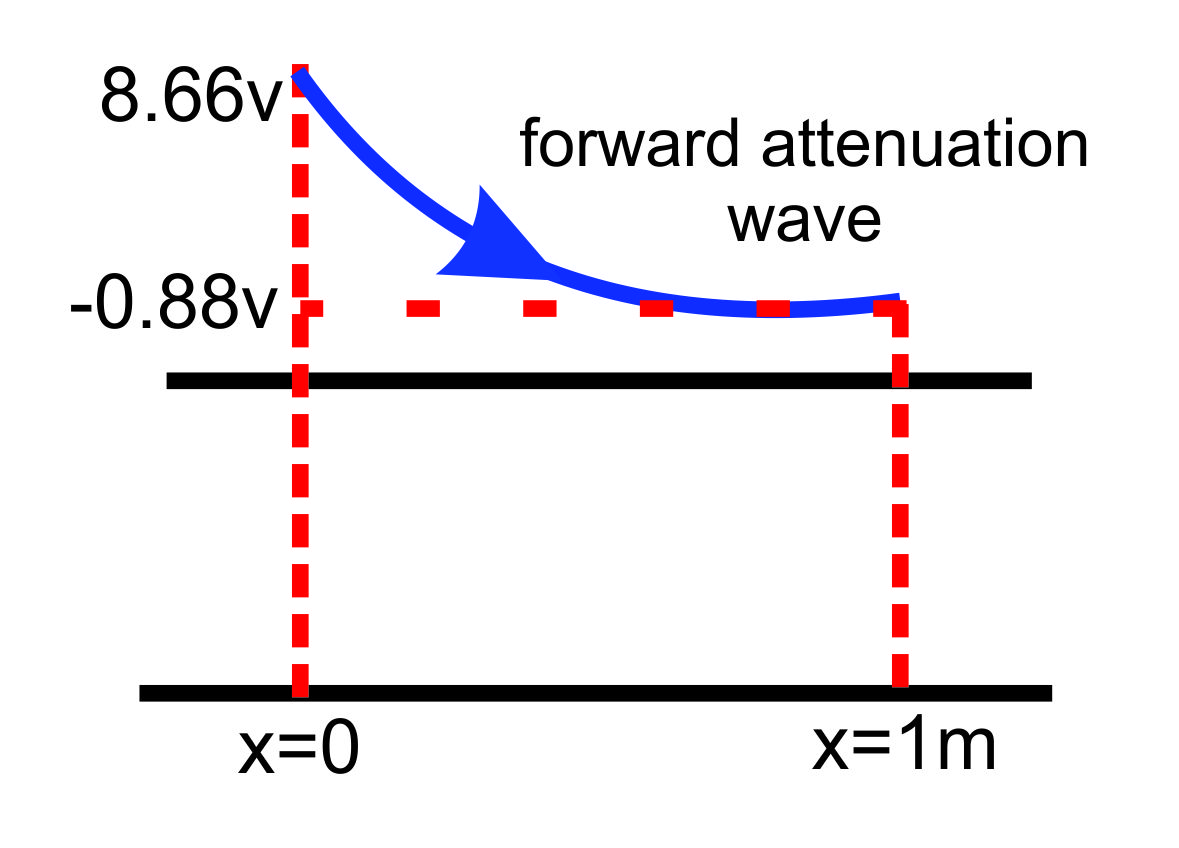
\includegraphics[scale=0.5]{./graphics/Group98}
\caption{Diagram for Problem 2}
\label{fig:group98}
\end{figure}

For the wave travelling in the negative direction, we have $V_{(x,t)} = \mathfrak{Re}\left\lbrace V^{-}e^{\gamma x}e^{j\omega t}\right\rbrace$ for backward wave.
\begin{dmath*}
V(x,t) = Re({V^{-}e^{\alpha x}e^{j\beta x}e^{j\omega t}}) = {|V^{-}|e^{\alpha x}cos{(\phi+\omega t + \beta x)}}
\end{dmath*}
At ${t=0, x=0, V=8.66}$, then
\begin{dmath*}
{8.66} = {|V^{-}|}e^{0} cos({\phi + 0 + 0})
= {|V^-|{cos\phi}} \quad \text{at }\phi\text{= 30\textdegree} 
= {|V^-|{cos30}}
= {|V^-|{0.866}}
\end{dmath*}
\begin{dmath*}
\frac{8.66}{0.866} = {|V^-|} = 10V
\end{dmath*}
\begin{align*}
V({x,t}) = 10e^{2.23x} \cos({\dfrac{\pi}{6} + 2\pi\times10^9t + 28.2x})
\end{align*}
At ${t=100nsec}$ and ${x=1m}$
\begin{dmath*}
V({x,t}) = 10e^{2.23} \cos({\dfrac{\pi}{6} + 2\pi\times10^9\times100\times10^{-9} + 28.2})
= -83.7701V
\end{dmath*}
So what we note here is, if we look at the transmission line with ${x=0}$ and ${x=1m}$. If the wave travels in forward direction, then the wave will attenuate in the direction of propagation. The variation is from ${8.66V}$ to ${-0.88V}$. In the backward direction, the wave will attenuate in the reverse direction so it has to  have a higher amplitude at ${x=1m}$ and ${t=100nsec}$ from were it attenuates from ${-83.7701V}$ to ${8.66V}$ in the other direction. The direction of propagation of the wave is very important.
\end{exmp}

\begin{exmp}
A transmision line has $L = 0.25muH/m$, $C=100pF/m$ and ${G=0}$. What should be the value of ${R}$ for the line so that the line can be travelled as a low loss line? The frequency of operation is ${100MHz}$

\subsection*{Solution}
For low loss line ${\alpha\ll\beta}$ say ${100\alpha=\beta}$ at 1 percent of ${\beta}$ value
\begin{dmath*}
\beta=\omega\sqrt{LC}
= {2\pi\times100\times10^6\sqrt{0.25\times10^{-6}\times100\times10^{-12}}}
=2\pi\times100\times10^6\times5\times10^{-9}
=\pi
\end{dmath*}
\begin{dmath*}
\alpha={\frac{1}{2}}\left(R\sqrt{\frac{C}{L}}+G\sqrt{\frac{L}{C}}\right)\quad (\text{G = 0})
={\frac{R}{2}}\sqrt{\frac{C}{L}}
=\frac{R}{2}\sqrt{\frac{100\times10^{-12}}{0.25\times10^{-6}}}
=\frac{R}{2}\sqrt{\frac{1}{2500}}
=\frac{R}{2}\times\frac{1}{50}
=\frac{R}{100}
\end{dmath*}
Remember ${\alpha = \frac{\beta}{100}}$, since ${\beta = \pi}$
\begin{dmath*}
\alpha = \frac{\beta}{100} 
= \frac{\pi}{100} 
= \frac{R}{100}
\end{dmath*}
\[\Longrightarrow R = \pi\Omega/m \]
So for this transmission line taking a resistance of ${3\Omega /m}$. It can be treated as a low loss transmission line. If ${R>\pi}$ say ${4\Omega}$, it is no more a low loss transmission line and it slowly become a lossy transmission line. When ${R}$ increases to the point that ${\alpha\approx\beta}$, then the line becomes extremely lossy.
\end{exmp}

So in this section, we have shown how to identify the load by looking at standing wave patterns. Next we solved some simple problems for transmission line based on voltage equations which we have derived for the transmission line. Next we go to applications of transmission line since we make use of sections of transmission line in realizing various circuit elements in high frequency circuits.
